\documentclass[10pt]{article}

\def\Type{LessonCaelan}
\def\TypeNum{Lesson 5}
\def\TypeTitle{Derivatives \& Rates of Change\\
Key }
\def\Semester{Fall 2021} %Not Used 
\def\Course{MATH 1190 \& 1210}
\def\Targets{ {\bf\color{ForestGreen}D1} }
\def\desmosClassCode{{\bf ZAJ$3$AZ}}
\usepackage{preambleDJ}

\usetikzlibrary{decorations.pathreplacing,angles,quotes}


%%%%%%%%%%%% BEGIN DOCUMENT %%%%%%%%%%%%%%%
%%%%%%%%%%%% BEGIN DOCUMENT %%%%%%%%%%%%%%%
%%%%%%%%%%%% BEGIN DOCUMENT %%%%%%%%%%%%%%%
%%%%%%%%%%%% BEGIN DOCUMENT %%%%%%%%%%%%%%%
%%%%%%%%%%%% BEGIN DOCUMENT %%%%%%%%%%%%%%%

\begin{document}

\pagestyle{otherpages}
\thispagestyle{firstpage}
\vs{.4}

\textbf{Intended Learning Outcomes}
After this lesson, you will be able to 

\begin{itemize}
    \item Describe the relationship between the derivative, slope of the tangent line, instantaneous rate of change, and average rate of change. (\target{D1})
    \item Explain the meaning of the derivative of a function at a given point in context, including determining the units of the derivative. (\target{D1})
    \item Identify and give examples of where a function might not be differentiable graphically. (\target{D1})
    \item Determine the sign and compare derivatives based on the graph. (\target{D1})
\end{itemize}

\vspace{-0.5cm}

\hrulefill


{\bf\color{blue}Warm-up} \exercise{\target{F1}}  Let $f(t)$ represent the distance travelled (in meters) by a skater around a track at a time $t$ in minutes. {\bf In this exercise, we want to learn about the skater's instantaneous velocity at time $t=3$ minutes.} Since we don't know how to compute this, we'll estimate with average velocity.\\

    \,\hfill
    \mpageT{.45}{.55}{\centering
    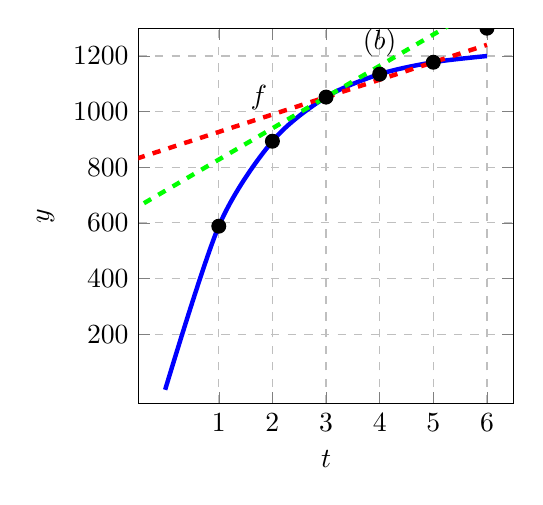
\begin{tikzpicture}[scale=1]
      \begin{axis}[
        xlabel={$t$},
        xtick       = {1,2,3,4,5,6},
        xticklabels = {$1$,$2$,$3$,$4$,$5$,$6$},
        ylabel={$y$},
        ytick       = {200,400,600,800,1000,1200},
        yticklabels = {$200$,$400$,$600$,$800$,$1000$,$1200$},
        samples     = 1280,
        domain      = -2:6,
        %restrict y to domain=-2:6,
        xmin = -0.5, xmax = 6.5,
        ymin = -50, ymax = 1300,
        width = 2.5in, height = 2.5in,
        grid=both, grid style=dashed
      ]
      \node at (1.75,1050) {$f$};
      % Original curve
%      \addplot[blue, ultra thick, mark=none, smooth] coordinates{ (0,0) (1,600) (2,894.43) (3,1039.23) (4,1131.37) (5,1183.22) (6,1200)};
%      \filldraw (1,600) circle (2.5pt);
%       \filldraw (2,894.43) circle (2.5pt);
%       \filldraw (3,1039.23) circle (2.5pt);
%       \filldraw (4,1131.37) circle (2.5pt); 
%       \filldraw (5,1183.22)  circle (2.5pt);  
%              \filldraw  (6,1200) circle (2.5pt); 
%%%%%%%%%%%%%%%
%%%%%%% Curve that works better with Desmos%%%%%%%%
      \addplot[blue, ultra thick, mark=none, smooth] coordinates{ (0,0) (1,588.17) (2,893.72) (3,1052.44) (4,1134.9) (5,1177.74) (6,1200)};
        \addplot[domain=-2:6, red, dashed,  ultra thick, mark=none] {62.65*(x-3)+1052.44};
           \addplot[domain=-2:6, green, dashed,  ultra thick, mark=none] {112.39*(x-3)+1052.44};
             \node at (4,1250) {\blue{$(b)$}};
      \filldraw (1,588.17) circle (2.5pt);
       \filldraw (2,893.72) circle (2.5pt);
       \filldraw (3,1052.44) circle (2.5pt);
       \filldraw (4,1134.9) circle (2.5pt); 
       \filldraw (5,1177.74)  circle (2.5pt);  
              \filldraw  (6,1300) circle (2.5pt); 
      % tangent line
      %\addplot[domain=-2:6, red, ultra thick, mark=none] {(x-.25)+.5};
      % secant line
      %\addplot[domain=0.25:1, ForestGreen, ultra thick, mark=none] {0.5/0.75*(x-1)+1};
      %\filldraw[black] (1,1) circle (2.5pt);
      % marking x-a
      %\draw[dashed] (1,.5) -- (.25,.5);
      %\node at (.625,.4) {$\Delta x$};
      % marking f(x)-f(a)
      %\draw[dashed] (1,.5) -- (1,1);
      %\node at (1.1,.75) {$\Delta y$};
      % cleaning up the image a bit
      %\filldraw[black] (0.25,0.5) circle (2.5pt);
    \end{axis}
    \end{tikzpicture}
}{
The data in this table  is plotted on the graph on the left.   \\ 
You might find the Desmos activity ``Skater, Derivatives and Rates of Change" at \href{https://student.amplify.com/}{student.amplify.com} helpful (see To Do or Past Work tab). Please use code \desmosClassCode.\\\\
%%%%%%% Data for original curve%%%%%%%%
%    \begin{tabular}{| l | l |}
%    \hline
%    $t$ & $f(t)$\\
%    \hline\hline
%    1 & 600\\
%    2 & 894.43\\
%    3 & 1039.23\\
%    4 & 1131.37\\
%    5 & 1183.22\\
%    6 & 1200\\
%    \hline
%    \end{tabular}
%%%%%%%%%%%%%%%%
%%%%%% Data that better fits Desmos curve %%%%%%
 \begin{tabular}{| l | l |}
    \hline
    $t$ & $f(t)$\\
    \hline\hline
    1 & 588.17\\
    2 & 893.72\\
    3 & 1052.44\\
    4 & 1134.9\\
    5 & 1177.74\\
    6 & 1200\\
    \hline
    \end{tabular}
}
    \hfill\,

  \enumA{
    \item Use a calculator (or Desmos) to compute the skater's average velocity from $3$ minutes to $t$ minutes after the start of the run. Round your answers to 2 decimal places.
  
    \begin{center}
    \begin{tabular}{| >{\centering\arraybackslash}m{1in} || >{\centering\arraybackslash}m{1in} | >{\centering\arraybackslash}m{1in} |>{\centering\arraybackslash}m{1in} |>{\centering\arraybackslash}m{1in} |>{\centering\arraybackslash}m{1in} |}
    \hline
    $t$ & $1$ & $2$ & $3$ & $4$ & $5$\\
    \hline
  \rule{0pt}{25pt}  $\displaystyle\frac{f(t)-f(3)}{t-3}$ \vfill&\blue{$232.14$}   & \blue{$158.72$}  &  {\large\color{blue} undefined}  &\blue{$82.46$}   &\blue{$62.65$} \\
    \hline
    \end{tabular}\\[0.25in]
    \end{center}



%\end{enumerate}\end{document} %end here for written preclass


    
    \item How can we represent these average velocities in the graph above? Draw something that represents the average velocity from $3$ minutes to $5$ minutes you found in part (b). Label this drawing with ``(b)". Use a straightedge (e.g. ID card) if you need to sketch any lines. \\
    \ep  Write down an equation for the object you sketched in part b) and graph it in Desmos. You will want to go to \href{https://student.amplify.com/}{student.amplify.com}  and use code \desmosClassCode.  
    \sol{
   Equation of line could be $y=62.65(t-3)+1052.44$ or $y=62.65(t-5)+1177.74$ or $y=62.65t+864.49.$ See red dashed line on graph above.
    }
    
    \item The table of values you wrote on the previous page in part (a) could be used to crudely estimate a limit. Which limit could it be used to estimate? You don't need to find the value of the limit - just write it.\\
    \mpageT{.4}{.6}{
    {\Large $\displaystyle\lim_{t\to\unline{.35}{\blue{$3$}}{.125}}\unline{2}{\blue{$\dfrac{f(t)-f(3)}{t-3}$}}{.4}$}
    }{ \large \blue{or $\ds \lim_{h\to0} \frac{f(t+h)-f(3)}{h} =\lim_{\Delta t\to0} \frac{f(t+\Delta t)-f(3)}{\Delta t}$ }
}
    
    \item In terms of the context described above, what does the limit you wrote in part (c) represent? ({\it Hint:} Lesson 1.)\\
\sol{The instantaneous velocity of the skater $3$ minutes after beginning to skate around the track}

    
    \item In terms of the graph above, what does the limit you wrote in part (c) represent?  ({\it Hint:} Lesson 1.)\\
\sol{The slope of the tangent line to the graph of $f$ at the point $t=3$.  See green dashed line on graph above. }

}

%%%%%%%%%
\newpage%
%%%%%%%%%

\,\\[-0.5in]

{\bf\color{blue} Mini-lecture.}  {\it Derivatives \& Differentiability}\\

The \href{https://www.desmos.com/calculator/kt2isjbgnr}{\bf Derivative} of a function $f$ at a number $a$ is denoted by $f'(a)$ and represents:
    \begin{enumerate}
    \item[i.] the \underline{slope of the tangent line} to the graph of $f$ at the point where $x=a$; and
    \item[ii.] the \underline{instantaneous rate of change} of $f$ in the instant when the input $x=a$.
    \end{enumerate}
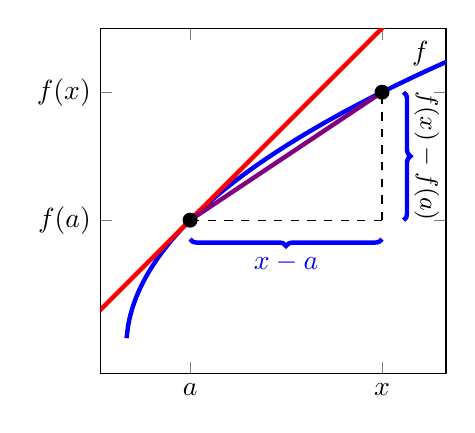
\begin{tikzpicture}[scale=1]
  \begin{axis}[
    %xlabel={$x$},
    xtick       = {.25,1},
    xticklabels = {$a$,$x$},
    ytick       = {.5,1},
    yticklabels = {$f(a)$,$f(x)$},
    samples     = 1280,
    domain      = -2:6,
    restrict y to domain=-2:6,
    xmin = -0.1, xmax = 1.25,
    ymin = -0.1, ymax = 1.25,
    width = 2.35in, height = 2.35in
  ]
  \node at (1.15,1.15) {$f$};
  \draw[blue, ultra thick, decoration={brace,mirror,raise=5pt},decorate]
  (.25,.48) -- node[below=6pt] {$x-a$} (1,.48);
  \draw[blue, ultra thick, decoration={brace,mirror,raise=5pt},decorate]
  (1.03,.5) -- node[right=5pt] {$$} (1.03,1);
  \node[rotate=-90] at (1.175,0.75) {\blue{\small$f(x)-f(a)$}};
  % curve
  \addplot[domain=-2:6, blue, ultra thick, mark=none] {x^(1/2)};
  % tangent line
  \addplot[domain=-2:6, red, ultra thick, mark=none] {(x-.25)+.5};
  % secant line
  \addplot[domain=0.25:1, violet, ultra thick, mark=none] {0.5/0.75*(x-1)+1};
  \filldraw[black] (1,1) circle (2.5pt);
  % marking x-a
  \draw[dashed] (1,.5) -- (.25,.5);
  %\node at (.625,.4) {$\Delta x$};
  % marking f(x)-f(a)
  \draw[dashed] (1,.5) -- (1,1);
  %\node at (1.1,.75) {$\Delta y$};
  % cleaning up the image a bit
  \filldraw[black] (0.25,0.5) circle (2.5pt);
\end{axis}
\end{tikzpicture}
%
\hfill\hfill\hfill
%
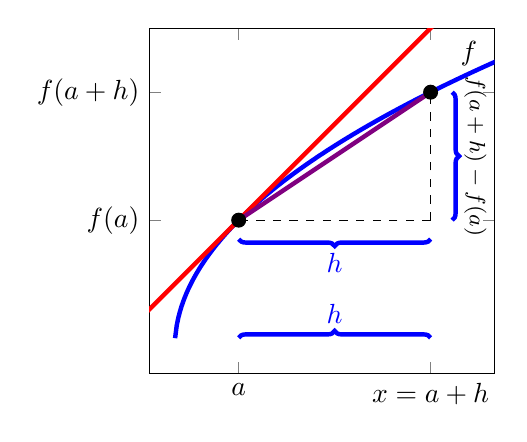
\begin{tikzpicture}[scale=1]
  \begin{axis}[
    %xlabel={$x$},
    xtick       = {.25,1},
    xticklabels = {$a$,$x=a+h$},
    ytick       = {.5,1},
    yticklabels = {$f(a)$,$f(a+h)$},
    samples     = 1280,
    domain      = -2:6,
    restrict y to domain=-2:6,
    xmin = -0.1, xmax = 1.25,
    ymin = -0.1, ymax = 1.25,
    width = 2.35in, height = 2.35in
  ]
  \node at (1.15,1.15) {$f$};
    \draw[blue, ultra thick, decoration={brace,mirror,raise=5pt},decorate]
  (.25,.48) -- node[below=6pt] {$h$} (1,.48);
   \draw[blue, ultra thick, decoration={brace,raise=0pt},decorate]
  (.25,.04) -- node[above=1pt] {$h$} (1,.04);
  \draw[blue, ultra thick, decoration={brace,mirror,raise=5pt},decorate]
  (1.03,.5) -- node[right=5pt] {$$} (1.03,1);
  \node[rotate=-90] at (1.175,0.75) {\blue{\footnotesize$f(a+h)-f(a)$}};
  % curve
  \addplot[domain=-2:6, blue, ultra thick, mark=none] {x^(1/2)};
  % tangent line
  \addplot[domain=-2:6, red, ultra thick, mark=none] {(x-.25)+.5};
  % secant line
  \addplot[domain=0.25:1, violet, ultra thick, mark=none] {0.5/0.75*(x-1)+1};
  \filldraw[black] (1,1) circle (2.5pt);
  % marking x-a
  \draw[dashed] (1,.5) -- (.25,.5);
  %\node at (.625,.4) {$\Delta x$};
  % marking f(x)-f(a)
  \draw[dashed] (1,.5) -- (1,1);
  %\node at (1.1,.75) {$\Delta y$};
  % cleaning up the image a bit
  \filldraw[black] (0.25,0.5) circle (2.5pt);
\end{axis}
\end{tikzpicture}\hfill\hfill\,\\

\hspace{0.5in} \fbox{$f'(a)=\displaystyle\lim_{x\to a}\frac{f(x)-f(a)}{x-a}$} \hfill\hfill \fbox{$f'(a)=\displaystyle\lim_{h\to0}\frac{f(a+h)-f(a)}{h}$} \hfill\,\\[0.1in]

As we have learned, sometimes limits do not exist. Accordingly, because the derivative is defined by a limit, sometimes derivatives do not exist! When the limit defining the derivative $f'(a)$ does exist, we say that $f$ is {\bf differentiable} at $a$. Here are some examples depicting where a function might \underline{not} be differentiable:\\

\,\hfill\hfill
%
\begin{minipage}[t][2.4in]{0.25\textwidth}
    %\begin{center}
        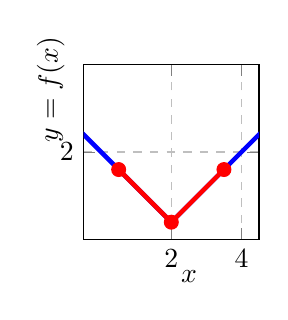
\begin{tikzpicture}[scale=1]
        \begin{axis}[
        %    axis y line = left,
        %    axis x line = bottom,
            xlabel={$x$},
            xlabel style={anchor= west},
            ylabel={$y=f(x)$},
            ylabel style={anchor= west},
            xtick       = {2,4},
            xticklabels = {$2$,$4$},
            ytick       = {2},
            yticklabels = {$2$},
            samples     = 160,
            domain      = -1:5,
            restrict y to domain=-1:5,
            xmin = -0.5, xmax = 4.5,
            ymin = -0.5, ymax = 4.5,
            grid=both, grid style=dashed,
            width=1.5in, height=1.5in
          ]
          % pieces 1 and 2
          \addplot[domain=-1:5, blue, ultra thick, mark=none] {abs(x-2)};
          \addplot[domain=.5:2, red, ultra thick, mark=none] {-x+2};
          \addplot[domain=2:3.5, red, ultra thick, mark=none] {x-2};
            \filldraw[red] (2,0) circle (2.5pt);
                \filldraw[red] (.5,1.5) circle (2.5pt);
                   \filldraw[red] (3.5,1.5) circle (2.5pt);
        \end{axis}
        \end{tikzpicture}\\[-0.15in]
        
        \,\quad\quad{\bf corners}
    %\end{center}
    \sol{
\itemCNIN{
    \item Slope of secant line on left is $-1$
       \item Slope of secant line on right is $+1$ 
       \item $2$-sided limit DNE. Thus $f^{\prime}(2)$ DNE.
}
}
\end{minipage}
%
\hfill
%
\vline
%
\hfill
%
\begin{minipage}[t][2.4in]{0.4\textwidth}
    \begin{center}
        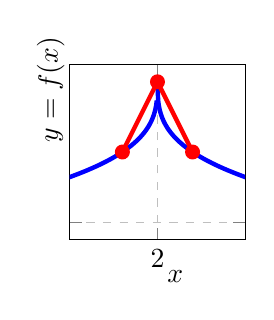
\begin{tikzpicture}[scale=1]
        \begin{axis}[
        %    axis y line = left,
        %    axis x line = bottom,
            xlabel={$x$},
            xlabel style={anchor= west},
            ylabel={$y=f(x)$},
            ylabel style={anchor= west},
            xtick       = {2},
            xticklabels = {$2$},
            ytick       = {0},
            yticklabels = {},
            samples     = 160,
            domain      = -1:5,
            restrict y to domain=-1:5,
            xmin = -0.5, xmax = 4.5,
            ymin = -0.5, ymax = 4.5,
            grid=both, grid style=dashed,
            width=1.5in, height=1.5in
          ]
          % pieces 1 and 2
          \addplot[domain=2:5, blue, ultra thick, mark=none] {4-2*abs((x-2)^(1/3))};
          \addplot[domain=-1:2, blue, ultra thick, mark=none] {4-2*abs((2-x)^(1/3))};
            \addplot[domain=1:2, red, ultra thick, mark=none] {2*x};
          \addplot[domain=2:3, red, ultra thick, mark=none] {-2*x+8};
            \filldraw[red] (2,4) circle (2.5pt);
                \filldraw[red] (1,2) circle (2.5pt);
                   \filldraw[red] (3,2) circle (2.5pt);
        \end{axis}
        \end{tikzpicture}\\
        {\bf vertical tangents}
    \end{center}
    \vs{-.3}
        \sol{
\itemCNIN{
    \item Slope of secant line on left is $+$ and growing towards $\infty$
   \item Slope of secant line on right is $-$ and growing towards $\infty$
       \item $2$-sided limit DNE. Thus $f^{\prime}(2)$ DNE.
}
}
\end{minipage}
%
\hfill
%
\vline
%
\hfill
%
\begin{minipage}[t][2.4in]{0.25\textwidth}
    \begin{flushright}
        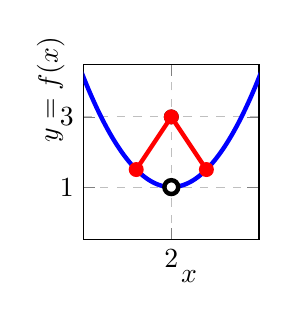
\begin{tikzpicture}[scale=1]
        \begin{axis}[
        %    axis y line = left,
        %    axis x line = bottom,
            xlabel={$x$},
            xlabel style={anchor= west},
            ylabel={$y=f(x)$},
            ylabel style={anchor= west},
            xtick       = {2},
            xticklabels = {$2$},
            ytick       = {1,3},
            yticklabels = {$1$,$3$},
            samples     = 320,
            domain      = -1:5,
            restrict y to domain=-1:5,
            xmin = -0.5, xmax = 4.5,
            ymin = -0.5, ymax = 4.5,
            grid=both, grid style=dashed,
            width=1.5in, height=1.5in
          ]
          % pieces 1 and 2
          \addplot[domain=-1:5, blue, ultra thick, mark=none] {1+(x-2)^2/2};
          \filldraw[white] (2,1) circle (2.5pt);
          \draw[ultra thick] (2,1) circle (2.5pt);
          \filldraw (2,3) circle (2.5pt);
            \addplot[domain=1:2, red, ultra thick, mark=none] {1.5*x};
          \addplot[domain=2:3, red, ultra thick, mark=none] {-1.5*x+6};
            \filldraw[red] (2,3) circle (2.5pt);
                \filldraw[red] (1,1.5) circle (2.5pt);
                   \filldraw[red] (3,1.5) circle (2.5pt);
        \end{axis}
        \end{tikzpicture}\\
        {\bf discontinuities}
    \end{flushright}
   \vs{-.3}
    \sol{
\itemCNIN{
    \item Slope of secant line on left is $+$ 
   \item Slope of secant line on right is $-$ 
       \item $2$-sided limit DNE. Thus $f^{\prime}(2)$ DNE.
}
}

\end{minipage}
%
\hfill\hfill\,

\example{\color{ForestGreen}D1} / \exercise{\color{ForestGreen}D1} Use the graphs of $f$ and $g$ below to find the following derivatives:
\vs{-.15}\\
\mpageTth{.45}{.3}{.3}{
%\begin{minipage}[t]{0.35\textwidth}
%\,\\[-0.1in]
    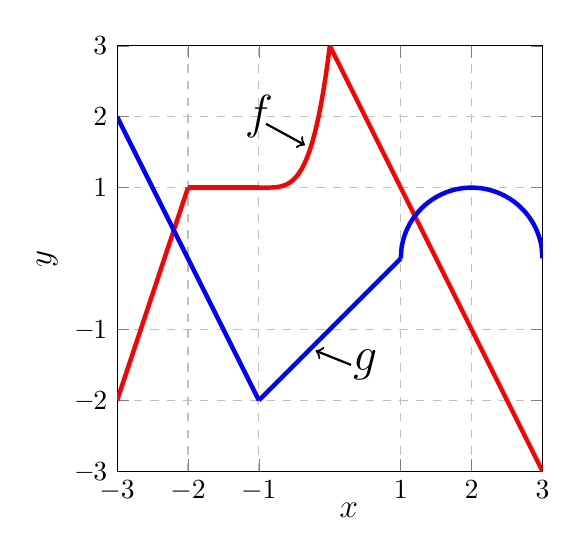
\begin{tikzpicture}[]
          \begin{axis}[
        %    axis y line = left,
        %    axis x line = bottom,
            xlabel = {\large$x$},
                            xlabel style={anchor=west},
            ylabel = {\large$y$},
                            ylabel style={anchor=south},
            xtick       = {-3,-2,-1,1,2,3},
            xticklabels = {$-3$,$-2$,$-1$,$1$,$2$,$3$},
            ytick       = {-3,-2,-1,1,2,3},
            yticklabels = {\textbf{--}$3$,\textbf{--}$2$,\textbf{--}$1$,$1$,$2$,$3$},
            samples     = 160,
            domain      = 0:3,
            restrict y to domain=-10:100,
            xmin = -3, xmax = 3,
            ymin = -3, ymax = 3,
            width=2.75in,height=2.75in,
            grid=both, grid style=dashed
          ]
          %
          \addplot[domain=-1:0, red, ultra thick, mark=none] {2*(x+1)^4+1};
          %
          \addplot[domain=-2:-1, red, ultra thick, mark=none] {1};
          %
          \addplot[domain=-3:-2, red, ultra thick, mark=none] {3*(x+2)+1};
          %
          \addplot[domain=0:3, red, ultra thick, mark=none] {-2*x+3};
          %
          \filldraw[black] (-1,2) circle (0pt) node[] {\LARGE $f$};
          %
          \draw[->,thick] (-0.9,1.9) -- (-0.35,1.6);
          %
          \addplot[domain=1:3, blue, ultra thick, mark=none] {(1-(x-2)^2)^(1/2)};
          %
          \addplot[domain=-1:1, blue, ultra thick, mark=none] {x-1};
          %
          \addplot[domain=-3:-1, blue, ultra thick, mark=none] {-2*(x+2)};
          %
          \filldraw[black] (0.5,-1.5) circle (0pt) node[] {\LARGE $g$};
          %
          \draw[->,thick] (0.3,-1.5) -- (-0.2,-1.3);
          %
        \end{axis}
    \end{tikzpicture}
%\end{minipage}
}{
%
%\hfill
%
%\begin{minipage}[t][2.5in]{0.3\textwidth}
    {\bf\color{blue}Examples.} \xdef\vsp{.4}
    \begin{enumerate}
    \item[(a)] $f'(1)=\dotfill$  \unline{.5}{\blue{$-2$}}{.15}
\vs{\vsp}
    \item[(b)] $f'(-1)=\dotfill$  \unline{.5}{\blue{$0$}}{.15}
\vs{\vsp}
    \item[(c)] $f'(0)=\dotfill$  \unline{.5}{\blue{$DNE$}}{.15}
\vs{\vsp}
    \end{enumerate}
%\end{minipage}
%%
%\hfill
%%
}{
%\begin{minipage}[t][2.5in]{0.3\textwidth}
    {\bf\color{blue}Exercises.}
    \begin{enumerate}
    \item[(a)] $g'(2)=\dotfill$  \unline{.5}{\blue{$0$}}{.15}
\vs{\vsp}
    \item[(b)] $g'(-1)=\dotfill$  \unline{.5}{\blue{$DNE$}}{.15}
\vs{\vsp}
    \item[(c)] $g'(-2)=\dotfill$  \unline{.5}{\blue{$-2$}}{.15}
\vs{\vsp}
    \end{enumerate}
%\end{minipage}
}


%%%%%%%%%
\newpage%
%%%%%%%%%
\vs{-.3}
\mpageTth{.55}{.25}{.25}{
%\begin{minipage}{0.525\textwidth}
\exercise{\color{ForestGreen}D1} The graph of $f$ is depicted to the right.
\enumA{
\item Use the graph of $f'$ to record some values of $f'$ \\in the table below.
}
\begin{tabular}{ c | p{0.6in} p{0.4in} p{0.6in} p{0.4in} }
& & & & \\
$x$ & $0<x<1$ & $x=1$ & $1<x<2$ & $x=2$\\
& & & & \\
\hline
& & & & \\
$f'(x)$ &\blue{$0$} & \blue{$DNE$} &  \blue{$-1$}&\blue{$DNE$} \\
& & & & \\
\end{tabular}
%\end{minipage}
}{
%
%\hfill
%%
%\begin{minipage}{0.45\textwidth}
    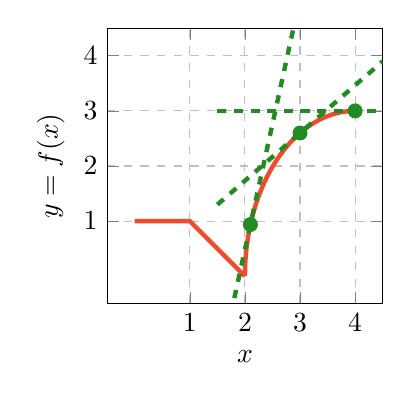
\begin{tikzpicture}[scale=1]
          \begin{axis}[
        %    axis y line = left,
        %    axis x line = bottom,
            xlabel={$x$},
            ylabel={$y=f(x)$},
            xtick       = {1,2,3,4},
            xticklabels = {$1$,$2$,$3$,$4$},
            ytick       = {1,2,3,4},
            yticklabels = {$1$,$2$,$3$,$4$},
            samples     = 320,
            domain      = -1:5,
            restrict y to domain=-1:5,
            xmin = -0.5, xmax = 4.5,
            ymin = -0.5, ymax = 4.5,
            grid=both, grid style=dashed,
            width=2in, height=2in
          ]
          % pieces 1 and 2
          \draw[RedOrange, ultra thick] (0,1) -- (1,1) -- (2,0);
          %\draw[RedOrange, ultra thick] (0,1) -- (1,1) -- (2,0) -- (3,3) -- (4,4);
          % piece 3
          \addplot[domain=2:4, RedOrange, ultra thick, mark=none] {(9-9/4*(x-4)^2)^(1/2)};
            \addplot[domain=1.5:3, dashed, ForestGreen, ultra thick, mark=none] {-8.64692+4.56365*x};
            \filldraw[ForestGreen] (2.1,.93675) circle (2.5pt);
             \addplot[domain=1.5:4.5, dashed, ForestGreen, ultra thick, mark=none] {sqrt(3)/2*x};
            \filldraw[ForestGreen] (3,2.5981) circle (2.5pt);
                 \addplot[domain=1.5:4.5, dashed, ForestGreen, ultra thick, mark=none] {3};
            \filldraw[ForestGreen] (4,3) circle (2.5pt);
          % label
        \end{axis}
    \end{tikzpicture}
%    %
%    \hfill
%    %
}{
    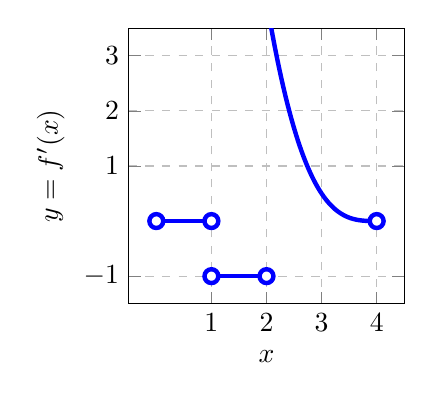
\begin{tikzpicture}[scale=1]
          \begin{axis}[
        %    axis y line = left,
        %    axis x line = bottom,
            xlabel={$x$},
                                    ylabel={$y=f^{\prime}(x)$},
            xtick       = {1,2,3,4},
            xticklabels = {$1$,$2$,$3$,$4$},
            ytick       = {-1,1,2,3},
            yticklabels = {$-1$,$1$,$2$,$3$},
            samples     = 320,
            domain      = -1:5,
            restrict y to domain=-1:5,
            xmin = -0.5, xmax = 4.5,
            ymin = -1.5, ymax = 3.5,
            grid=both, grid style=dashed,
            width=2in, height=2in
          ]
                    \draw[blue, ultra thick] (0,0) -- (1,0) ;
                    \draw[blue, ultra thick] (1,-1) -- (2,-1) ;
          %\draw[RedOrange, ultra thick] (0,1) -- (1,1) -- (2,0) -- (3,3) -- (4,4);
          % piece 3
          \addplot[domain=2:4, blue, ultra thick, mark=none] {4/8*(4-x)^3};
                  \filldraw[white] (0,0) circle (2.5pt);
          \draw[blue, ultra thick] (0,0) circle (2.5pt);
                    \filldraw[white] (1,0) circle (2.5pt);
          \draw[blue, ultra thick] (1,0) circle (2.5pt);
                              \filldraw[white] (1,-1) circle (2.5pt);
          \draw[blue, ultra thick] (1,-1) circle (2.5pt);
                              \filldraw[white] (2,-1) circle (2.5pt);
          \draw[blue, ultra thick] (2,-1) circle (2.5pt);
                                        \filldraw[white] (4,0) circle (2.5pt);
          \draw[blue, ultra thick] (4,0) circle (2.5pt);
        \end{axis}
    \end{tikzpicture}
%\end{minipage}\\
}
\enumA{\setItemnumber{2}
\item  Use the graph of $f$ and the table you built in part (a) to sketch the graph of $f'$ in the empty grid above for $0\leq x \leq 4$.
\sol{
\itemI{
\item Derivatives do not exist at $x=1$ and $x=2$ because of corners on original graph. This is represented on blue graph with a hole.  
\item We're not sure what's going on with graph at $x=0$ without more information. Thus we're not sure if derivative exists at $x=0$, hence the hole at $x=0$. The same is true at $x=4$.
\item The tangent lines just to the right of $x=2$ are very steep. They flatten out as $x\to4$, thus derivative approaches $0$.Thus the function we draw just to the right of $x=2$ should have large values that decrease to $0$. One (of many) reasonable examples is shown.
}
}
}
\begin{minipage}[t]{0.75\textwidth}
\exercise{\color{ForestGreen}D1} A {\bf cost curve} is a graph depicting the relationship between the total cost $C$ of producing a quantity $Q$ of a particular commodity. The cost curve for a particular commodity is given to the right.

\begin{enumerate}

\item[(a)] What does $\dfrac{C(400)-C(200)}{400-200}$ represent in this context? Sketch a line whose slope would represent this quantity geometrically in the grid to the right.
\sol{
This fraction represents the average rate of change of the total cost ($C$) of production as quantity ($Q$) in creases from $200$ to $400$.  This is average increase in total cost per $1$ unit increase in production between $200$ and $400$ units of production. \\\\
The slope of the blue secant line on the graph is this same quantity
}
\end{enumerate}
\end{minipage}
%
\hfill
%
\begin{minipage}[t]{0.2\textwidth}
\begin{center}
        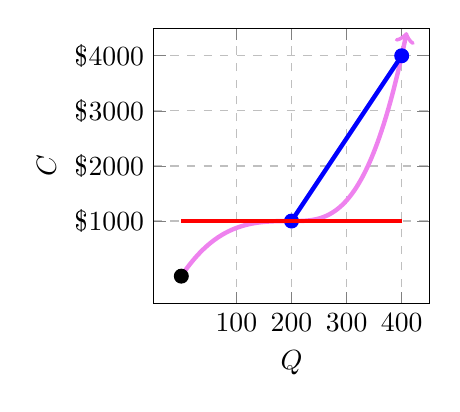
\begin{tikzpicture}[scale=1]
            \begin{axis}[
                %    axis y line = left,
                %    axis x line = bottom,
                    xlabel={$Q$},
                    xtick       = {100,200,300,400},
                    xticklabels = {100,200,300,400},
                    ylabel={$C$},
                    ytick       = {1000,2000,3000,4000},
                    yticklabels = {\$1000,\$2000,\$3000,\$4000},
                    samples     = 160,
                    domain      = -50:450,
                    restrict y to domain=-500:4500,
                    xmin = -50, xmax = 450,
                    ymin = -500, ymax = 4500,
                    grid=both, grid style=dashed,
                    width=2in, height=2in
                  ]
                  %\addplot[Violet, ultra thick, smooth] coordinates{ (0,0) (100,70) (200,1000) (300,1250) (400,4000) };
                  \addplot[Violet, ultra thick,domain=0:200] {(x-200)^3/8000+1000};
                  \addplot[Violet, ultra thick, domain=200:450,->] {(x-200)^3*3/8000+1000};
                        \draw[blue, ultra thick] (200,1000) -- (400,4000) ;
                    \filldraw[blue] (200,1000) circle (2.5pt);
                    \filldraw[blue] (400,4000) circle (2.5pt);
                  \filldraw (0,0) circle (2.5pt);
                     \draw[red, ultra thick] (0,1000) -- (400,1000) ;
            \end{axis}
        \end{tikzpicture}
\end{center}
\end{minipage}

\vfill

\begin{enumerate}

\item[(b)] What are the units of measurement of the quantity $\dfrac{C(400)-C(200)}{400-200}$? $\dotfill$ \unline{1.75}{\blue{$\dfrac{\$}{\text{units of }Q}$}}{.35}

\item[(c)] What does $\displaystyle\lim_{Q\to200}\dfrac{C(Q)-C(200)}{Q-200}$ represent in this context? Sketch a line whose slope would represent this quantity geometrically in the grid above.

\sol{
This limit represents the instantaneous rate of change of the total cost of production ($C$) when $200$ units of $Q$ are produced. This is expected increase in total cost per $1$ unit increase in production if costs continues to change exactly as it did when $200$ units were produced.\\\\
In economics, this quantity is {\em  marginal cost}.\\\\
The slope of the red tangent line on the graph is this same limit.
}

\item[(d)] What are the units of measurement of the quantity $\displaystyle\lim_{Q\to200}\dfrac{C(Q)-C(200)}{Q-200}$? \unline{1.75}{\blue{$\dfrac{\$}{\text{units of }Q}$}}{.35}

\end{enumerate}

%%%%%%%%%
\newpage%
%%%%%%%%%

{\bf\color{blue}Extra Practice 1.}\reversemarginpar\marginnote{\fbox{\bf\color{ForestGreen}D1}} A particle travels along the $x$-axis such that its position (in centimeters) along the axis at time $t$ (in seconds) is given by the function $p(t)$. Click the {\color{blue}\href{https://www.geogebra.org/classic/z4pka8p6}{\bf \underline{link}}} (either on this lesson or on Canvas) to see the particle's motion over the time interval $0 < t < 6$. 

\begin{enumerate}

\item[(a)] What are the units of measurement of $p'(t)$?  \unline{2.5}{\blue{$\dfrac{\text{centimeters}}{\text{second}}$}}{.35}

\item[(b)] Write a sentence describing what $p'(t)$ represents in this context.\\ 
({\bf Note:} ``in this context" means your answer must clearly relate to the scenario described in the problem - a supply curve relating position $p$ and time $t$. Answers like ``the derivative of $p$" are not in this context.)

\sol{
The instantaneous velocity of the particle at time $t$seconds;. The particle is traveling $p^{\prime}(t)\;cm/sec$ at time $t$  seconds.
}

\item[(c)] Based on the animation, for which values of $t$ is the derivative $p'(t)$ Positive? Negative? Zero? Explain your thoughts. 
  
    \begin{enumerate}
    \item[i.] positive?  \blue{$0<t<2$ since particle is moving to the right (i.e. in positive direction) during this time interval.}\\
    \item[ii.] negative?\blue{$2<t<6$ since particle is moving to the left (i.e. in negative direction) during this time interval.}\\
    \item[iii.] zero?  \blue{$t=2$ since particle transitions from positive velocity (i.e. to the right) to negative velocity (i.e. moving to the left).}
    \end{enumerate}

\end{enumerate}



{\bf\color{blue}Extra Practice 2.}\reversemarginpar\marginnote{\fbox{\bf\color{ForestGreen}D1}} The curve below gives the mass $m(t)$ (in grams) of a substance at a time $t$ (in seconds) during a chemical reaction. Arrange the following quantities from least to greatest:
\begin{itemize}
\item {\bf Quantity A:} the rate at which the mass of the substance is changing at time $t=1$
\item {\bf Quantity B:} the rate at which the mass of the substance is changing at time $t=2$
\item {\bf Quantity C:} the rate at which the mass of the substance is changing at time $t=3$
\item {\bf Quantity D:} $0$
\end{itemize}

\begin{center}
\begin{minipage}{0.45\textwidth}
\begin{center}
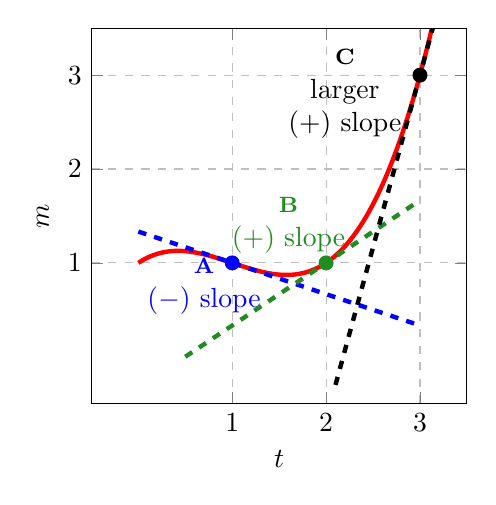
\begin{tikzpicture}[scale=1]
  \begin{axis}[
%    axis y line = left,
%    axis x line = bottom,
    xtick       = {1,2,3},
    xticklabels = {$1$,$2$,$3$},
    xlabel      = {$t$},
    ytick       = {1,2,3},
    yticklabels = {$1$,$2$,$3$},
    ylabel      = {$m$},
    samples     = 160,
    domain      = 0:4.5,
    restrict y to domain=-10:100,
    xmin = -0.5, xmax = 3.5,
    ymin = -0.5, ymax = 3.5,
    grid=both, grid style=dashed,
    width=2.5in, height=2.5in
  ]
  %
  %\addplot[blue, ultra thick, mark=none, smooth] coordinates{ (0,1) (0.5,1.25) (1,1) (1.5,0.75) (2,1) (2.5,1.5) (3,3)};
  \addplot[red, ultra thick, mark=none] {(x)*(x-1)*(x-2)/3+1};
    \addplot[blue, dashed, ultra thick, mark=none, domain=0:3] {(4-x)/3};
    \filldraw[blue] (1,1) circle (2.5pt);
    \node[align=center, blue] at (.7,.75) {\footnotesize {\bf A} \\ $(-)$ slope}; 
        \addplot[ForestGreen, dashed, ultra thick, mark=none, domain=.5:3] {1/3*(2*x-1)};
    \filldraw[ForestGreen] (2,1) circle (2.5pt);
        \node[align=center, ForestGreen] at (1.6,1.4) {\footnotesize {\bf B} \\ $(+)$ slope}; 
     \addplot[black, dashed, ultra thick, mark=none, domain=2.1:3.5] {-8+11*x/3};
    \filldraw[black] (3,3) circle (2.5pt);
            \node[align=center, black] at (2.2,2.8) {\footnotesize {\bf C} \\ larger\\ $(+)$ slope}; 
  %\addplot[name path=g, domain=-1:3.5, black, thick, mark=none, ] {0.5*e^x};
  %
\end{axis}
\end{tikzpicture}
\end{center}
\end{minipage}
%
\quad
%
\begin{minipage}{0.45\textwidth}
\,\hfill
{\Large \unline{.4}{\blue{\bf A}}{.25}\textless\,\unline{.4}{{\bf D}}{.25} \textless\, \unline{.4}{\fgreen{\bf B}}{.25} \textless\, \unline{.4}{\bf C}{.25}}\hfill\,\\

\,\hfill{\scriptsize (example answer format: D \textless\, C \textless\, B \textless\, A) }\hfill\,
\end{minipage}
\end{center}
\sol{
\itemI{
\item Tangent line {\bf A} at $x=1$ has a $(-)$ slope.
\item Tangent line {\bf B} at $x=2$ has a $(+)$ slope.
\item Tangent line {\bf C} at $x=3$ has a $(+)$ slope. Slope is even greater than at $x=2$
\item This leads to {\bf A} $< ${\bf D}$=0<${\bf B}$<${\bf C}
}
}
\newpage
{\bf\color{blue}Extra Practice 3.}\reversemarginpar\marginnote{\fbox{\bf\color{ForestGreen}D1}} Pictured below are pairs of graphs. Choose the letter if the corresponding pair is the graph of a function $f$ and its derivative $f'$. (One or more of the choices below may be correct.) \\

%\includegraphics[scale=0.7]{Spring 2021/Classwork (S21)/Classwork 4.1/MultSelect}

    \,\hfill
    \begin{minipage}[t]{0.2\textwidth}
        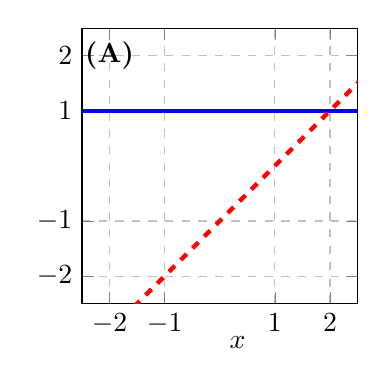
\begin{tikzpicture}[scale=1]
          \begin{axis}[
        %    axis y line = left,
        %    axis x line = bottom,
            xlabel={$x$},
                        xlabel style={anchor=west},
            xtick       = {-2,-1,1,2},
            xticklabels = {$-2$,$-1$,$1$,$2$},
            ytick       = {-2,-1,1,2},
            yticklabels = {$-2$,$-1$,$1$,$2$},
            samples     = 320,
            domain      = -3:3,
            restrict y to domain=-3:3,
            xmin = -2.5, xmax = 2.5,
            ymin = -2.5, ymax = 2.5,
            grid=both, grid style=dashed,
            width=2in, height=2in
          ]
          % graph 1
          \draw[blue, ultra thick] (-3,1) -- (3,1);
          % graph 2
          \addplot[domain=-3:3, red, dashed, ultra thick, mark=none] {x-1};
          % label
          \node at (-2,2) {\bf (A)};
        \end{axis}
        \end{tikzpicture}
    \end{minipage}
    %
    \hfill
    %
    \begin{minipage}[t]{0.2\textwidth}
        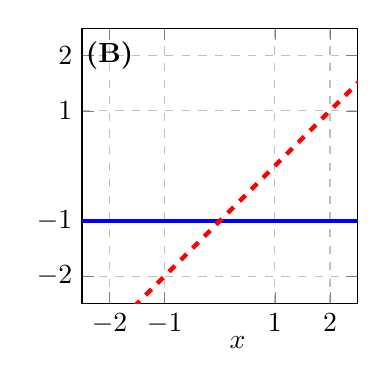
\begin{tikzpicture}[scale=1]
          \begin{axis}[
        %    axis y line = left,
        %    axis x line = bottom,
            xlabel={$x$},
                        xlabel style={anchor=west},
            xtick       = {-2,-1,1,2},
            xticklabels = {$-2$,$-1$,$1$,$2$},
            ytick       = {-2,-1,1,2},
            yticklabels = {$-2$,$-1$,$1$,$2$},
            samples     = 320,
            domain      = -3:3,
            restrict y to domain=-3:3,
            xmin = -2.5, xmax = 2.5,
            ymin = -2.5, ymax = 2.5,
            grid=both, grid style=dashed,
            width=2in, height=2in
          ]
          % graph 1
          \draw[blue, ultra thick] (-3,-1) -- (3,-1);
          % graph 2
          \addplot[domain=-3:3, red, dashed, ultra thick, mark=none] {x-1};
          % label
          \node at (-2,2) {\bf (B)};
        \end{axis}
        \end{tikzpicture}
    \end{minipage}
    %
    \hfill
    %
    \begin{minipage}[t]{0.2\textwidth}
        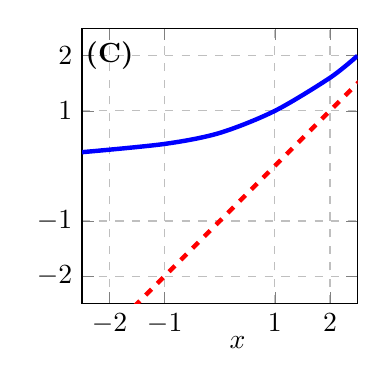
\begin{tikzpicture}[scale=1]
          \begin{axis}[
        %    axis y line = left,
        %    axis x line = bottom,
            xlabel={$x$},
                        xlabel style={anchor=west},
            xtick       = {-2,-1,1,2},
            xticklabels = {$-2$,$-1$,$1$,$2$},
            ytick       = {-2,-1,1,2},
            yticklabels = {$-2$,$-1$,$1$,$2$},
            samples     = 320,
            domain      = -3:3,
            restrict y to domain=-3:3,
            xmin = -2.5, xmax = 2.5,
            ymin = -2.5, ymax = 2.5,
            grid=both, grid style=dashed,
            width=2in, height=2in
          ]
          % graph 1
          \addplot[blue, ultra thick, smooth] coordinates{(-2.5,0.25) (-1,0.4) (0,0.6) (1,1) (2,1.6) (2.5,2)};
          % graph 2
          \addplot[domain=-3:3, red, ultra thick, dashed, mark=none] {x-1};
          % label
          \node at (-2,2) {\bf (C)};
        \end{axis}
        \end{tikzpicture}
    \end{minipage}
    %
    \hfill
    %
    \begin{minipage}[t]{0.2\textwidth}
        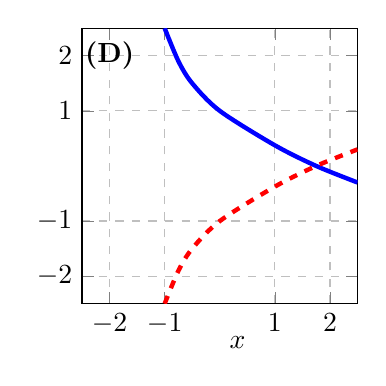
\begin{tikzpicture}[scale=1]
          \begin{axis}[
        %    axis y line = left,
        %    axis x line = bottom,
            xlabel={$x$},
                        xlabel style={anchor=west},
            xtick       = {-2,-1,1,2},
            xticklabels = {$-2$,$-1$,$1$,$2$},
            ytick       = {-2,-1,1,2},
            yticklabels = {$-2$,$-1$,$1$,$2$},
            samples     = 320,
            domain      = -3:3,
            restrict y to domain=-3:3,
            xmin = -2.5, xmax = 2.5,
            ymin = -2.5, ymax = 2.5,
            grid=both, grid style=dashed,
            width=2in, height=2in
          ]
          % graph 1
           \addplot[blue, ultra thick, smooth] coordinates{(-1,2.5) (-0.75,1.9) (-0.5,1.5) (0,1) (1,0.375) (1.75,0) (2.5,-0.3)};

          % graph 2
          \addplot[red, ultra thick, dashed, smooth] coordinates{(-1,-2.5) (-0.75,-1.9) (-0.5,-1.5) (0,-1) (1,-0.375) (1.75,0) (2.5,0.3)};
          % label
          \node at (-2,2) {\bf (D)};
        \end{axis}
        \end{tikzpicture}
    \end{minipage}
    \hfill\,\\
\sol{
\enumA{
\item[\bf (A)]  {\bf YES} this is  an example of graph of $f$ and graph of $f^{\prime}$. Here's why.
\itemI{
\item If $f(x)$ is the red dashed line, then since it's a linear function, it has a constant positive slope. It looks like this slope is about $1$.  
\item Thus $f^{\prime}(x) =1$ for all $x$
\item Blue solid line is the graph of $y=1$ and could be a graph of $f^{\prime}$.
\item So {\bf YES}, if we assume $f(x)$ is the red dashed line then $f^{\prime}(x)$ could be the blue solid line and this is example of graph of $f$ and graph of $f^{\prime}$.
}
\item[\bf (B)] {\bf NO} this is not an example of graph of $f$ and graph of $f^{\prime}$. Here's why.
\itemI{
\item If $f(x)$ is red dashed line, then $f^{\prime}(x) =1$ as in (A).  Blue solid line is graph of $y=-1$, so this cannot be $f^{\prime}(x)$
\item If $f(x)$ is blue solid line, it has a slope of $0$ everywhere and thus $f^{\prime}(x)=0$.  But red dashed line is not constantly $0$, so it cannot be $f^{\prime}(x)$.
\item Thus, no matter what we assume about $f(x)$, the graph of the other function cannot be $f^{\prime}(x)$.
}
\item[\bf (C)] {\bf NO} this is not an example of graph of $f$ and graph of $f^{\prime}$. Here's why.
\itemI{
\item If we assume $f(x)$ is red dashed line, it has a constant slope of about $1$ and thus $f^{\prime}(x)=1$ for all $x$. The graph of the blue solid line is {\em not} the graph of $y=1$ and thus it cannot be $f^{\prime}(x)$.
\item If we assume that $f(x)$ is blue solid line, we notice that this function is increasing. That means all tangent lines will have positive slope and $f^{\prime}(x)>0$ for all $x$.  Red dashed line is negative for $x<1$ and thus it cannot be $f^{\prime}(x)$.
\item Thus, no matter what we assume about $f(x)$, the graph of the other function cannot be $f^{\prime}(x)$.
}
\item[\bf (D)] {\bf NO} this is not an example of graph of $f$ and graph of $f^{\prime}$. Here's why.
\itemI{
\item If we assume $f(x)$ is red dashed line, we notice that it's always increasing. This means all tangent lines will have a positive slope and thus  $f^{\prime}(x)>0$ for all $x$.   But blue solid line turns negative at around $x=1.75$. So it cannot be $f^{\prime}(x)$.
\item If we assume that $f(x)$ is blue solid line, we notice that this function is decreasing.  That means all tangent lines will have negative slope and $f^{\prime}(x)<0$ for all $x$. But red dashed line becomes positive at around$x=1.75$ so it cannot be $f^{\prime}(x)$.
\item Thus, no matter what we assume about $f(x)$, the graph of the other function cannot be $f^{\prime}(x)$.
}
}
}
\end{document}
